%%%%%%%%%%%%%%%%%%%%%%%%%%%%%%%%%%%%%%%%%%%%%
%                Rubens Braz                %
%            www.rubensbraz.com             %
%%%%%%%%%%%%%%%%%%%%%%%%%%%%%%%%%%%%%%%%%%%%%

% Definições Iniciais --------------------------------------------------
\documentclass[12pt]{report}

%\usepackage[a4paper]{geometry}
\usepackage[left=2.8cm, right=2.8cm, top=4cm]{geometry} % margens da folha

\usepackage[utf8]{inputenc} % caracteres com acento

\usepackage[english,portuguese]{babel}
\usepackage[T1]{fontenc} %tradução

\usepackage{url} % exibição de URL's

\usepackage{subfigure}
\usepackage{graphicx, multicol, latexsym, amsmath, amssymb} % permite inserção de imagens e fórmulas matemáticas

\graphicspath{{../pdf/}{../jpeg/}}
\DeclareGraphicsExtensions{.pdf,.jpeg,.png} % formatos aceitos

\usepackage{hyphenat} % hífens; veja a última linha antes do início do documento, corrigir erros de hifenização lá!

\usepackage{etoolbox}
\apptocmd{\sloppy}{\hbadness 10000\relax}{}{} % remove erros de underfull hbox em links

\usepackage{color} % permite a mudança de cor do texto

\usepackage{xcolor,soul,framed}
\colorlet{shadecolor}{yellow} % define cor do destacado como amarelo

\usepackage{silence}
\WarningFilter{caption}{Unsupported document class} % remove o erro no pacote 'caption'
\usepackage{caption} % permite a inserção de legendas em imagens

\usepackage{eqparbox} % facilita a criação de grupos

\usepackage{listings} % permite a escrita de códigos de programação

\usepackage{indentfirst} % identação depois de uma seção

\usepackage{tabularx} % tabelas com tamanho variável de coluna

\usepackage{array}

\makeatletter
\patchcmd{\chapter}{\if@openright\cleardoublepage\else\clearpage\fi}{}{}{}
\makeatother % Manter capítulos na mesma página

\hyphenation{matemá-tica} % corrigir erros de hifenização aqui!

\usepackage{placeins}

% Início do documento --------------------------------------------------
\begin{document}

% Cabeçalho
\begin{center}
    \vspace*{-3cm}
    \textsc{Universidade de Brasília} \\
    \textsc{Faculdade de Tecnologia}
    
    \vspace{1cm}
    \rule{411pt}{1.3pt}
    \vspace{0.2cm}
    
    \Large \textbf{\textsc{Aprendizado por Reforço na Geração de Marcha em Robô Quadrúpede}}
    
    \rule{411pt}{1.3pt}
    \vspace{1cm}
    
    Aluno: Rubens Saito Mira Braz\\
    \vspace{0.5cm}
    Pesquisador Responsável: Alexandre Ricardo Soares Romariz
    
    \vspace{1cm}
\end{center}


% Resumo
\vspace*{-0.5cm}
\section*{Resumo}

Este projeto de pesquisa explora o Aprendizado por Reforço para melhoria de marchas de um robô quadrúpede. Tais marchas são geradas por parâmetros e, com um algoritmo em Python que interpreta notas, foi possível obter uma melhoria de pouco mais de 30\% na distância percorrida.


% Introdução
\vspace*{-0.6cm}
\chapter*{Introdução}

\vspace*{-0.75cm}
\section*{Contextualização}

Robôs quadrúpedes são estudados pelas suas diversas aplicações. A disposição das patas permite que essa classe de robôs consiga acessar áreas acidentadas e assim ajudar no resgate de vítimas. Além disso, o transporte de cargas também é bastante explorado já que a distribuição do peso se dá entre as patas, proporcionando um alívio sobre os motores.


\section*{Histórico da Plataforma e Objetivos}

Diversos trabalhos foram realizados desde 2006 para a implementação e aperfeiçoamento de um robô quadrúpede no Laboratório de Automação e Robótica (LARA) da Universidade de Brasília (UnB). Na tabela \ref{ultimos_projetos} são mostrados os últimos projetos feitos utilizando esse robô. Alguns dos principais objetos de estudo eram a robótica comportamental e a robótica terrestre.

\begin{table}[ht!]
\centering
\resizebox{\textwidth}{!}{%
\begin{tabular}{|l|l|l|}
\hline
Autores & Ano & Título \\ \hline
PORPHIRIO, C. de F.; SANTANA, P. H. M. & 2017 & \begin{tabular}[c]{@{}l@{}}Geração de marchas para a plataforma quadrúpede\\ utilizando algoritmo genético.\end{tabular} \\ \hline
FLORIANO, B. R de O. & 2017 & \begin{tabular}[c]{@{}l@{}}Desenvolvimento e interação de um sistema\\ de controle de equilíbrio para um robô quadrúpede.\end{tabular} \\ \hline
DOS SANTOS, P. M .F; DUARTE, V. A. & 2018 & \begin{tabular}[c]{@{}l@{}}Aprendizado de marchas factíveis para um robô \\ quadrúpede utilizando algoritmo genético multiobjetivo.\end{tabular} \\ \hline
BRAZ, JÚLIA CABRAL DINIZ & 2018 & \begin{tabular}[c]{@{}l@{}}Melhoramento de marcha para robô quadrúpede\\ utilizando estratégia de aprendizagem por reforço\end{tabular} \\ \hline
\end{tabular}%
}
\caption{Os mais recentes projetos desenvolvidos utilizando a plataforma quadrúpede do LARA.}
\label{ultimos_projetos}
\end{table}

Na figura \ref{historico}, podemos ver as várias versões da plataforma utilizada. Durante o desenvolvimento desse projeto, o robô usado é o da figura \ref{historico} c).

\begin{figure}[h!]
    \centering
    
    \subfigure[Primeira versão desenvolvida \cite{4}]{
    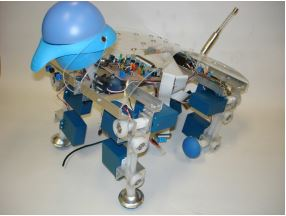
\includegraphics[height=3.5cm]{imagens/introducao/robo1.JPG}}
    \hfill
    \subfigure[Quadrúpede após o trabalho de Batista e Cardoso \cite{5}]{
    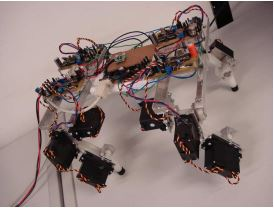
\includegraphics[height=3.5cm]{imagens/introducao/robo2.JPG}}
    \hfill
    \subfigure[Plataforma reestruturada por Santos \cite{6}]{
    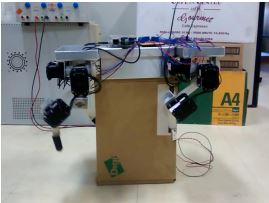
\includegraphics[height=3.5cm]{imagens/introducao/robo3.JPG}}
    
    \caption{Histórico do robô quadrúpede do LARA. \cite{7}}
    \label{historico}
\end{figure}


\section*{Aprendizado de Máquina}

Como Arthur Samuel definiu \cite{1}, aprendizado de máquina é o ``campo de estudo que dá aos computadores a habilidade de aprender sem serem explicitamente programados''. Isto é, utilizando algoritmos para coletar e aprender com os dados, podemos fazer previsões e melhorar comportamentos.


\section*{Definição do problema e Objetivo do Projeto}

Dos Santos e Duarte \cite{2} criaram em 2018 um modelo de marcha adequado ao funcionamento da plataforma quadrúpede utilizada nesse projeto. Essa marcha possui quatro poses, que são descritas por um conjunto de parâmetros.

Devido ao grande número de testes feitos no robô para a obtenção dos parâmetros ideais, esse projeto foca em utilizar formas mais eficiente de aprendizado, utilizando-se do mesmo modelo de marcha.


% Fundamentos Teóricos
\vspace*{-0.6cm}
\chapter*{Fundamentos Teóricos}

\vspace*{-0.75cm}
\section*{Aprendizado por reforço}

Aprendizado por reforço (RL, do inglês \textit{Reinforcement Learning}) é diferente de aprendizado supervisionado (AS). No AS, o agente aprende a partir de um conjunto de dados pré-determinados por um supervisor externo. Ou seja, as ações tomadas foram definidas anteriormente. O objetivo do RL é o agente generalizar sua resposta para situações que ainda não tenham sido programadas.

Pode-se imaginar que o RL é um aprendizado não-supervisionado pois ele não precisa de exemplos de comportamentos corretos, no entanto, esse tipo de algoritmo tenta maximizar um sinal de recompensa em vez de encontrar padrões.

Na maioria das vezes, projetos de pesquisa envolvendo RL usam o processo de decisão de Markov. Isto é, um agente - tomador de decisões - encontra uma situação para a qual ele ainda não foi testado. Logo, seu objetivo passa a ser encontrar uma sequencia de ações para operar o sistema de forma mais eficiente, com base em critérios de funcionamento previamente estabelecidos e levando em conta que o estado do sistema futuro à tomada de decisão depende do estado atual \cite{3}.

\section*{Estrutura do robô quadrúpede}

O robô possui uma estrutura de alumínio e patas de nylon. Sua estrutura é composta por quatro patas. Cada pata possui 3 servos motores, totalizando assim doze graus de liberdade de movimento.

A Figura \ref{estrutura} representa a localização dos servos motores na plataforma e a convenção adotada para nomenclatura das patas. Os servos utilizados são do modelo \textit{Dynamixel} RX-28 da \textit{Robotis}, a tensão de alimentação é de no mínimo 12 Volts, sendo 14,8 Volts a tensão recomendada pelo fabricante  \cite{8}. O torque máximo de servo é de 3,7 N.m.

\begin{figure}[ht!]
	\captionsetup{justification=centering}
	\centering
	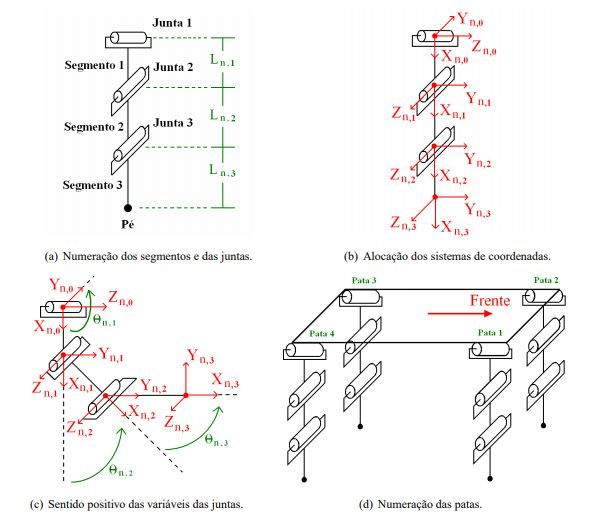
\includegraphics[width=0.7\linewidth]{imagens/fundamentos/cordpatas.JPG}
	\caption{Estrutura do quadrúpede \cite{9}.}
	\label{estrutura}
\end{figure}

\section*{Sensoriamento}

O sistema de sensoriamento do robô foi feito por Porphiro e Santana \cite{10}. Atualmente, o sistema do quadrúpede oferece medidas sobre a aceleração - utilizando-se um acelerômetro (modelo Digital ADXL345) - e medidas das forças nas extremidades das patas - utilizando-se um sensor resistivo de força (modelo FSR 400, possui resolução de 0,2N e atua entre 0,2 e 20N).

A informação sobre a força aplicada nas patas é relevante para se conhecer a carga que cada pata está submetida, além de mostrar o exato momento do toque da pata no chão.

O acelerômetro informa a orientação do centro de massa do quadrúpede, por conseguinte é possível saber se o mesmo está na trajetória definida. % Ademais, a estabilidade do robô é conseguida a partir do controle da rolagem e da arfagem do centro de massa da estrutura. Se o acelerômetro está parado e sem angulações de arfagem ou rolagem, a aceleração medida é de 1g no Eixo Y.

\section*{Sistemas embarcados}

O quadrúpede é controlado por uma integração entre \textit{Raspberry PI} e o \textit{Arduíno}, em uma relação mestre-escravo. O Arduíno coleta dados dos sensores de força e do acelerômetro e envia ao \textit{Raspberry PI}, via serial. O \textit{Raspberry PI} é responsável por controlar os servo motores a partir de um código em C++, com uma biblioteca da \textit{Dynamixel}, fabricante dos motores.

\section*{Definições da marcha e simulações}

O trabalho realizado de Dos Santos e Duarte \cite{2}, que utiliza algoritmo genético, encontrou 4 poses para as patas do quadrúpede utilizando cinemática inversa. Essas poses podem ser vistas na figura \ref{poses} e foram inspiradas em caminhadas de cavalos. 

Cada marcha para o quadrúpede é uma composição dessas 4 poses. E, além disso, cada pose é alterada por parâmetros (são 5 ao todo) - eles são: ângulos de aberturas das poses 2 ($angle-front$) e 3 ($angle-back$) e posição no espaço da extremidade durante pose de transição, pose 1 ($x_c, y_c, z_c$). Logo, os parâmetros são: $P=\{angle-front, angle-back, x_c, y_c, z_c\}$. 

\begin{figure}[h!]
\centering
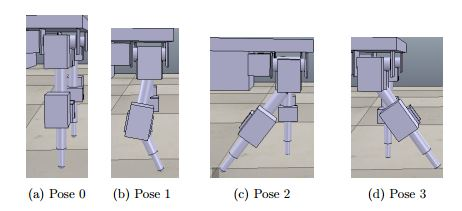
\includegraphics[scale=1]{imagens/fundamentos/poses.JPG}
\caption{Poses das patas geradas por cinemática inversa \cite{2}.}
\label{poses}
\end{figure}

Cada pata executa a seguinte sequência de poses durante uma marcha (a ordem das poses é chamada de ciclo e ele é repetido duas vezes):

\begin{itemize}
    \item \textbf{Pata 1:} Pose 3 $\rightarrow$ Pose 4 $\rightarrow$ Pose 1 $\rightarrow$ Pose 2;
    \item \textbf{Pata 2:} Pose 1 $\rightarrow$ Pose 2 $\rightarrow$ Pose 3 $\rightarrow$ Pose 4;
    \item \textbf{Pata 3:} Pose 3 $\rightarrow$ Pose 4 $\rightarrow$ Pose 1 $\rightarrow$ Pose 2;
    \item \textbf{Pata 4:} Pose 1 $\rightarrow$ Pose 2 $\rightarrow$ Pose 3 $\rightarrow$ Pose 4;
\end{itemize}

* A localização de cada pata na estrutura do robô pode ser vista na figura \ref{estrutura}.
\vspace{0.3cm}

O software \textit{V-REP} foi escolhido para simular o comportamento do robô pois ele se destaca por oferecer uma grande gama de técnicas de simulação e pela portabilidade de seus modelos e controladores \cite{10}. Além disso, ele também já havia sido adotado por Porphirio e Santana \cite{10} para simulação da plataforma quadrúpede e esse trabalho usou esse modelo já desenvolvido anteriormente.


% Metodologia
\vspace*{-0.6cm}
\chapter*{Metodologia}

\vspace*{-0.75cm}
\section*{Introdução}

Para a tentativa de melhora das marchas desenvolvidas por Dos Santos e Duarte \cite{2}, foram utilizados dois métodos diferentes de aprendizado por reforço. Na primeira tentativa, foi usado um algoritmo de diferença temporal com traço de elegibilidade, mas ao se mostrar demorado e não muito efetivo, outro algoritmo foi utilizado. Esta segunda tentativa é baseada no gradiente de política, que se mostrou mais rápido e eficaz. Sendo inclusive factível para aplicação direta no robô, sem antes passar por simulações.

\section*{Diferença temporal com traço de elegibilidade}

O modelo de robô quadrúpede usado nesse trabalho precisa aprender apenas os melhores valores para os parâmetros que geram as marchas. Considerando que o estado é um conjunto de parâmetros o importante é determinar qual o melhor estado (valores ótimos dos parâmetros), a ação a ser tomada em cada estado não é importante.

Para um teste de eficiência desse método, foi tentada a variação de apenas 3 dos 5 parâmetros que compões as marchas. Quando mais parâmetros são variados, maior é o espaço de estados e a análise se torna muito complexa e o tempo de simulação muito extenso. Cada parâmetro usado nesse algoritmo foi discretizado em um intervalo específico - isso é necessário para que o espaço de estados seja minimizado e também evitar valores que impeçam o correto funcionamento do robô.

Os valores de mínimo e máximo de cada parâmetro foi definido no trabalho de Dos Santos e Duarte \cite{2} - e os mesmos estão definidos abaixo:

\begin{itemize}
    \item $angle-back$ e $angle-front$: Estes parâmetros são os ângulos em que a pata do robô faz nas poses 2 e 3, que podem ser vistas na Figura \ref{poses}. Possuem valor de $30^{\circ}$, pois nas marchas obtidas por Dos Santos e Duarte \cite{2} eles se aproximavam deste valor;
    \item $x_c$: Representa a posição x que a extremidade da pata do robô deve alcançar durante a pose 1. Limitada no intervalo [17,21] cm, com um passo de 0,4.
    \item $y_c$: Representa a posição y que a extremidade da pata do robô deve alcançar durante a pose 1. Limitada no intervalo [-4,0] cm, com um passo de 0,4.
    \item $z_c$: Representa a posição z que a extremidade da pata do robô deve alcançar durante a pose 1. Limitada no intervalo [0,4] cm, com um passo de 0,4.
\end{itemize}

Na aplicação deste algoritmo, o problema de aprendizado é definido como um Processo de Decisão de Markov, que é composto de:

\begin{itemize}
    \item $S$: Estados $s$ que são um conjunto de parâmetros, $s(x_{c},y_{c}, z_{c})$;
    \item $A$: Ações $a(s)$: pode incrementar o valor de um parâmetro, decrementar o valor de um parâmetro, e continuar no mesmo estado.
    \item $T(s,a,s')$: Função de transição determinística que permite o incremento ou decremento de apenas um parâmetro e ainda permite o sistema ficar no mesmo estado.
    \item $r$: Uma recompensa negativa é dada ao robô quando ele falha em andar certa distância mínima, ou quando cai, e uma recompensa positiva é determinada como uma função da distância percorrida.  
\end{itemize}

Foi utilizado um algoritmo no MATLAB \cite{11} para otimizar esses parâmetros.

\section*{Gradiente de Política}

Utilizando o método de Diferença Temporal com Traço de Elegibilidade, foi constatado que o mesmo demorava exageradamente para encontrar os valores dos estados. Por isso, foi buscada uma alternativa mais eficaz. Foi adotado o método de Gradiente de Política, que além de mais eficaz, também não necessita da discretização dos parâmetros - ele também é capaz de trabalhar em grande espaço de estados.

Foi utilizado um algoritmo em \emph{MATLAB} baseado em um desenvolvido no trabalho de Kohl e Stone \cite{12}. Este método busca um máximo global, em contrapartida aos métodos de gradiente tradicionais, que buscam máximos locais.

O método utilizado pode ser considerado uma derivação dos métodos de gradiente de política padrões. Ao utilizarmos métodos de gradiente de política a convergência em busca da política ótima apenas se aproximará do máximo local, em contraste com a técnica utilizada no trabalho citado acima em que converge para um máximo global.

Nesta técnica, consideramos um vetor de parâmetros iniciais $P_{ini} = \{angle-back, angle-front, x_{c}, y_{c}, z_{c}\}$ e é estimada a derivada parcial da função objetivo de $P_{ini}$ em relação a cada parâmetro. Isso é feito primeiramente avaliando $n$ políticas próximas de $P_{ini}(R_1, R_2, \cdots , R_n)$, que são geradas aleatoriamente. Essas políticas são definidas como:

$$R_i = \{angle-back+\Delta_1 , angle-front+\Delta_2, x_c+\Delta_3, y_c+\Delta_4, z_c+\Delta_5\}$$

onde $\Delta_n$ é escolhido de modo aleatório entre três opções \{$+\epsilon_n ,0, -\epsilon_n$\}. Cada $\epsilon_n$ é um valor fixado de acordo com o parâmetro a qual ele está ligado. 

Uma nota ($score$) da marcha é atribuída para cada política. Essa nota pode ser tanto a distância percorrida por y, a variação no eixo x, a variação no eixo z, ou até mesmo uma média ponderada de todos estas medidas. A função objetivo pode ser maximizar, ou até mesmo minimizar, estes valores. 

Depois que todas as políticas são avaliadas são estimadas as derivadas parciais em relação a cada um dos 5 parâmetros. Isso é feito agrupando cada $R_i$ em um dos 3 conjuntos para cada umas das dimensões:
$$R_i \in \left \{
\begin{array}{ll}
S_{+\epsilon,n}, & \text{se o enésimo parâmetro de $R_i$ é $p_n + \epsilon_n$};\\
S_{0,n}, & \text{se o enésimo parâmetro de $R_i$ é $p_n + 0$};\\
S_{-\epsilon,n}, & \text{se o enésimo parâmetro de $R_i$ é $p_n -  \epsilon_n$}.\\
\end{array}
\right.$$

É computada então um nota média $Avg_{+\epsilon,n}$, $Avg_{0,n}$ e $Avg_{-\epsilon,n}$ para $S_{+\epsilon,n}$, $S_{0,n}$ e $S_{-\epsilon,n}$ respectivamente. Essas três médias representam qual é o beneficio de se alterar o enésimo parâmetro por $+\epsilon_n$, $0$ ou $-\epsilon_n$.

Essas médias são usadas para ajustar um vetor $A$ com 5 variáveis, onde:
$$A_n = \left \{
\begin{array}{cl}
0, & \text{se } Avg_{+0,n} >  Avg_{+\epsilon,n} \text{ e }  Avg_{+0,n} >  Avg_{-\epsilon,n};\\
Avg_{+\epsilon,n} - Avg_{-\epsilon,n}, & \text{caso contrário.}\\
\end{array}
\right.$$

O vetor $A$ é normalizado e multiplicado por um escalar de passo $\eta$, para que o ajuste seja constante (fixo) a cada iteração. Ao final adicionamos A ao vetor $P_{ini}$, e uma nova iteração é iniciada.

O algoritmo desenvolvido no \emph{MATLAB}, faz a cada iteração 5 avaliações de diferentes marchas. Como as simulações no \textit{V-REP} possuem muito ruído, cada marcha era simulada 3 vezes. A cada vez que o algoritmo era rodado eram feitas 10 iterações. O algoritmo foi rodado pelo menos duas vezes, e, se em uma nova rodada, pelo menos uma política teve $score$ maior que todas as políticas da rodada anterior, o algoritmo era rodado mais uma vez, caso contrário, ele não era mais iniciado e a política que obteve maior $score$ da vez anterior era considerada a política ótima. 

Vários objetivos diferentes foram testados nesse método de aprendizado \cite{7}:

\begin{itemize}
    \item Maximização da distância no eixo y. Para isso, o $score$ é considerado a distância total percorrida neste eixo.
    
    \item Minimização da variação no eixo z, ou seja, minimizar o balanço da altura do robô na tentativa de penalizar políticas em que o robô acaba por cair. Para isso o $score$ é o inverso da diferença entre o maior e menor valor lido pelo GPS no  eixo z de coordenadas. Se utiliza do inverso pois o algoritmo visa maximizar o $score$.
    
    \item Minimização da variação no eixo x, pois se deseja que o robô ande apenas no eixo y, se há uma diferença grande no eixo x que dizer que a marcha gerada pende para um algum lado. Utiliza-se novamente o inverso da diferença entre os valores máximo e mínimos lidos pelo GPS.
    
    %\item Maximização da média ponderada da distância percorrida em y, inverso da variação em z e inverso da variação em x. Neste caso buscamos que todas as características buscadas individualmente anteriormente sejam satisfeitas em uma única marcha.
\end{itemize}

O \emph{MATLAB}, que inicia a simulação no \emph{V-REP}, foi utilizado num primeiro momento para testar o algoritmo desenvolvido. Dado os bons resultados das simulações, o algoritmo foi reescrito em \emph{Python 3.6} para que ele fosse testado na plataforma real. O código em \emph{Python} gerava as marchas que o código em C++ executava.

% Resultados
\vspace*{-0.6cm}
\chapter*{Resultados - Gradiente de Política:}

\vspace*{-0.75cm}
\section*{Maximização da distância percorrida em y}

A princípio, a função objetivo foi apenas maximizar a distância percorrida no eixo $y$. Para começar a execução do algoritmo de gradiente de política, é necessário a escolha de uma política inicial, foi escolhida a marcha final obtida no trabalho de Dos Santos e Duarte (marcha que gera $61 cm$ de distância percorrida), pois a marcha achada por eles obtém resultados satisfatórios e a convergência desse algoritmo depende de um bom chute inicial.

A Figura \ref{fig:marcha1e5} apresenta os resultados de duas execuções do algoritmo sendo iniciando com os parâmetros obtidos por Dos Santos e Duarte \cite{2}. As iterações que possuem valor zero, revelam parâmetros incapazes de gerar marchas factíveis. Na Simulação 1, foram necessárias 20 iterações para se encontrar um valor máximo de $55 cm$. Na Simulação 5, foram necessárias 30 iterações e foi encontrado um valor máximo de $65 cm$.

\begin{figure}[ht!]
\centering
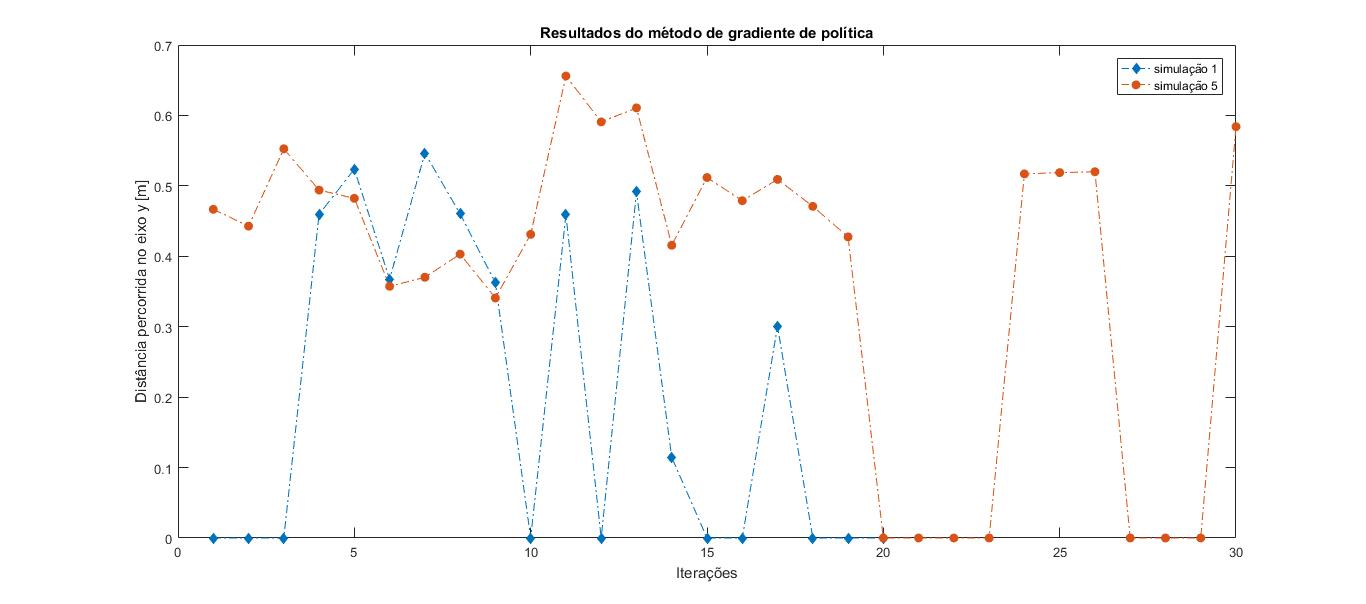
\includegraphics[width=0.9\textwidth]{imagens/resultados/marcha1e5.jpg}
\caption{Distância percorrida ao final de cada iteração da primeira e segunda execução do algoritmo.}
\label{fig:marcha1e5}
\end{figure}

Na terceira execução, foi adotada como política inicial os resultados obtidos na Simulação 5. Ao final, o resultado obtido foi uma distância total percorrida de $72 cm$. Isso mostra que ao se iniciar as iterações em políticas boas, é possível a obtenção de melhores resultados. Também podemos verificar que começar em políticas diferentes geram resultados diferentes, pois esse método encontra a política ótima local.

Esses resultados foram advindos de simulações no \emph{V-REP}, depois as marchas também foram testadas na plataforma real e os resultados foram bem próximos.

\begin{figure}[ht!]
\centering
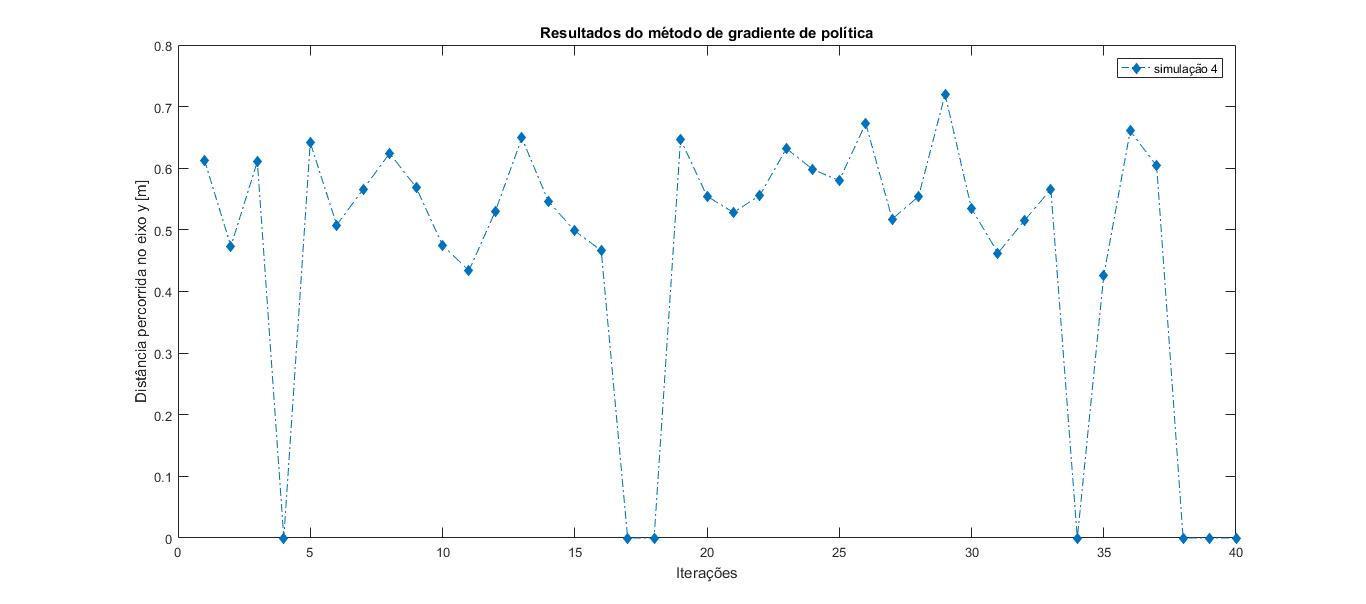
\includegraphics[width=0.9\textwidth]{imagens/resultados/marcha4.jpg}
\caption{Distância percorrida ao final de cada iteração da terceira execução do algoritmo.}
\label{fig:marcha4}
\end{figure}


% Conclusão
\vspace*{-0.6cm}
\chapter*{Conclusão}
\vspace*{-0.75cm}

Este trabalho foi capaz de usar a técnica de aprendizado por reforço para obter valores de parâmetros do gerador de marcha de um robô quadrúpede em um ambiente simulado. Para a otimização foram utilizados dois métodos diferentes.

O primeiro foi o de diferença temporal, onde os parâmetros da marcha são considerados o estado do robô. Neste método, o valor dos estados são aproximados conforme os estados são visitados e uma implementação com parâmetros contínuos seria inviável. 

Com as restrições impostas, para se obter uma estimativa da função valor eram necessárias muitas horas, cerca de 15. Os parâmetros foram discretizados a passos muito grandes e, sendo a marcha muito sensível a estes parâmetros, foi visto que outras algoritmos de aprendizado poderiam ser mais eficientes.

O segundo método utilizado foi o de gradiente de política. Nesse algoritmo, os parâmetros não são mais tidos como estados mas sim como uma política que o robô executa. Logo, o objetivo passa a ser encontrar a política ótima. 

Com esse segundo método, o tempo de simulação diminuiu bastante, passando a ser de 1:30h, e com poucas iterações foi possível a obtenção de resultados bem melhores. A marcha usada para inciar o algoritmo conseguia percorrer uma distância de $61 cm$ e a marcha final encontrada nesse trabalho chegou a andar $80 cm$ (ambas distâncias medidas na plataforma real), um aumento de mais de 30\%.

A desvantagem no uso deste segundo método está no fato de que, diferentemente do método utilizado anteriormente, a busca pelos melhores parâmetros converge apenas para um ótimo local.

A 'Marcha 0' é a que foi obtida no trabalho de Dos Santos e Duarte \cite{2}, e a 'Marcha 12' é a que obteve a maior distância percorrida.


% Bibliografia
\bibliography{references}

\begin{thebibliography}{12}

	\bibitem{1} SAMUEL, A. L. Some studies in machine learning using the game of checkers. IBM Journal ofresearch and development, IBM, v. 3, n. 3, p. 210–229, 1959.
	
	\bibitem{2} SANTOS, P. M. F. dos; DUARTE, V. A.Aprendizado de marcha para um robô quadrúpede utilizando algoritmo genético multiobjetivo. Monografia (Graduação) — Universidade de Brasília, Brasília, Julho 2018.
	
	\bibitem{3} PUTERMAN, M. L.Markov decision processes:  discrete stochastic dynamic programming. 1. ed. New Jersey:  Wiley-Interscience, 1994. (Wiley Series in Probability and Statistics). ISBN 0471619779,9780471619772.
	
	\bibitem{4} COTTA, G. H.; RAULINO NETO, L. Realização de uma plataforma para estudo de robótica comportamental baseada em quadrúpedes. Monografia (Graduação) — Universidade de Brasília, Brasília, 2006.
	 
	\bibitem{5} BATISTA, G. F.; CARDOSO, I. F. Adequação de um sistema de locomoção de um robô quadrúpede para avaliação de algoritmos de aprendizagem. Monografia (Graduação) — Universidade de Brasília, Brasília, 2007.
	 
	\bibitem{6} SANTOS, J. H. de S. Plataforma quadrúpede: Uma nova estrutura para robô quadrúpede do LARA. Monografia (Graduação) — Universidade de Brasília, Brasília, Julho 2016.

    \bibitem{7} BRAZ, JÚLIA CABRAL DINIZ. Melhoramento de marcha para robô quadrúpede utilizando estratégia de aprendizagem por reforço. Monografia (Graduação) — Universidade de Brasília, Brasília, Julho 2018.
    
    \bibitem{8} ROBOTICS.ROBOTIS E-Manual. Disponível em: \url{http://emanual.robotis.com/docs/en/software/rplus1/dynamixel\_wizard/}. Acesso em: 18 jun. 2019.
    
    \bibitem{9} SOUTO, R. F. Modelagem cinemática de um robô quadrúpede e geração de seus movimentos usando filtragem estocástica. Monografia (Graduação) — Universidade de Brasília, Brasília, Julho 2007.
    
    \bibitem{10} PORPHIRIO, C. de F.; SANTANA, P. H. M. Geração de marchas para a plataforma quadrúpede utilizando algoritmo genético. Monografia (Graduação) — Universidade de Brasília, Brasília, Junho 2017.
    
    \bibitem{11} MathWorks. MATLAB. Aplicativo para Windows 10.
    
    \bibitem{12} KOHL, N.; STONE, P. Policy gradient reinforcement learning for fast quadrupedal locomotion. In: IEEE.Robotics and Automation, 2004. Proceedings. ICRA’04. 2004 IEEE International Conference. New Orleans, 2004.
    
\end{thebibliography}

\end{document}